\documentclass{article}
\usepackage[utf8]{inputenc}
\usepackage[spanish]{babel} 


\usepackage{graphicx} %paquete básico para incluir gráficos
\usepackage{wrapfig} %paquete Wrapfig
\usepackage{float} % paquete para controlar entornos flotantes
\usepackage{pdfpages}% Paquete pdfpages incluye páginas completas de ficheros pdfs
\usepackage{lipsum} % Paquete para introducir texto 
%
\usepackage{tikz} % Paquete TikZ para generar gráficos
\usetikzlibrary{babel,shapes,arrows}


\title{Taller LaTeX Yosigopublicando: Graficos}
\author{ossanche }
\date{March 2021}

\begin{document}

\maketitle

\section{Inclusión de gráficos}

%%%%%%%%%%%%%%%%%%%%%%%%%%%%%%%%%%%%%%%%
\lipsum % incluimos texto
{\bf Final lipsum 1}

\begin{figure}[h]
    \centering
    
\includegraphics[height=5cm,angle=30]{graficos/ciclista.jpeg}
    \caption{Gráfico simple insertado. \LaTeX lo coloca donde estima oportuno.}
    \label{fig:1}
\end{figure}

Así esta figura puede ser referenciada haciendo una llamada a su etiqueta como se puede apreciar en Figura \ref{fig:1}.

%%%%%%%%%%%%%%%%%%%%%%%%%%%%%%%%%%%%%%%%
\lipsum % incluimos texto
{\bf Final lipsum 2}

\begin{figure}[h]
    \centering
    \frame{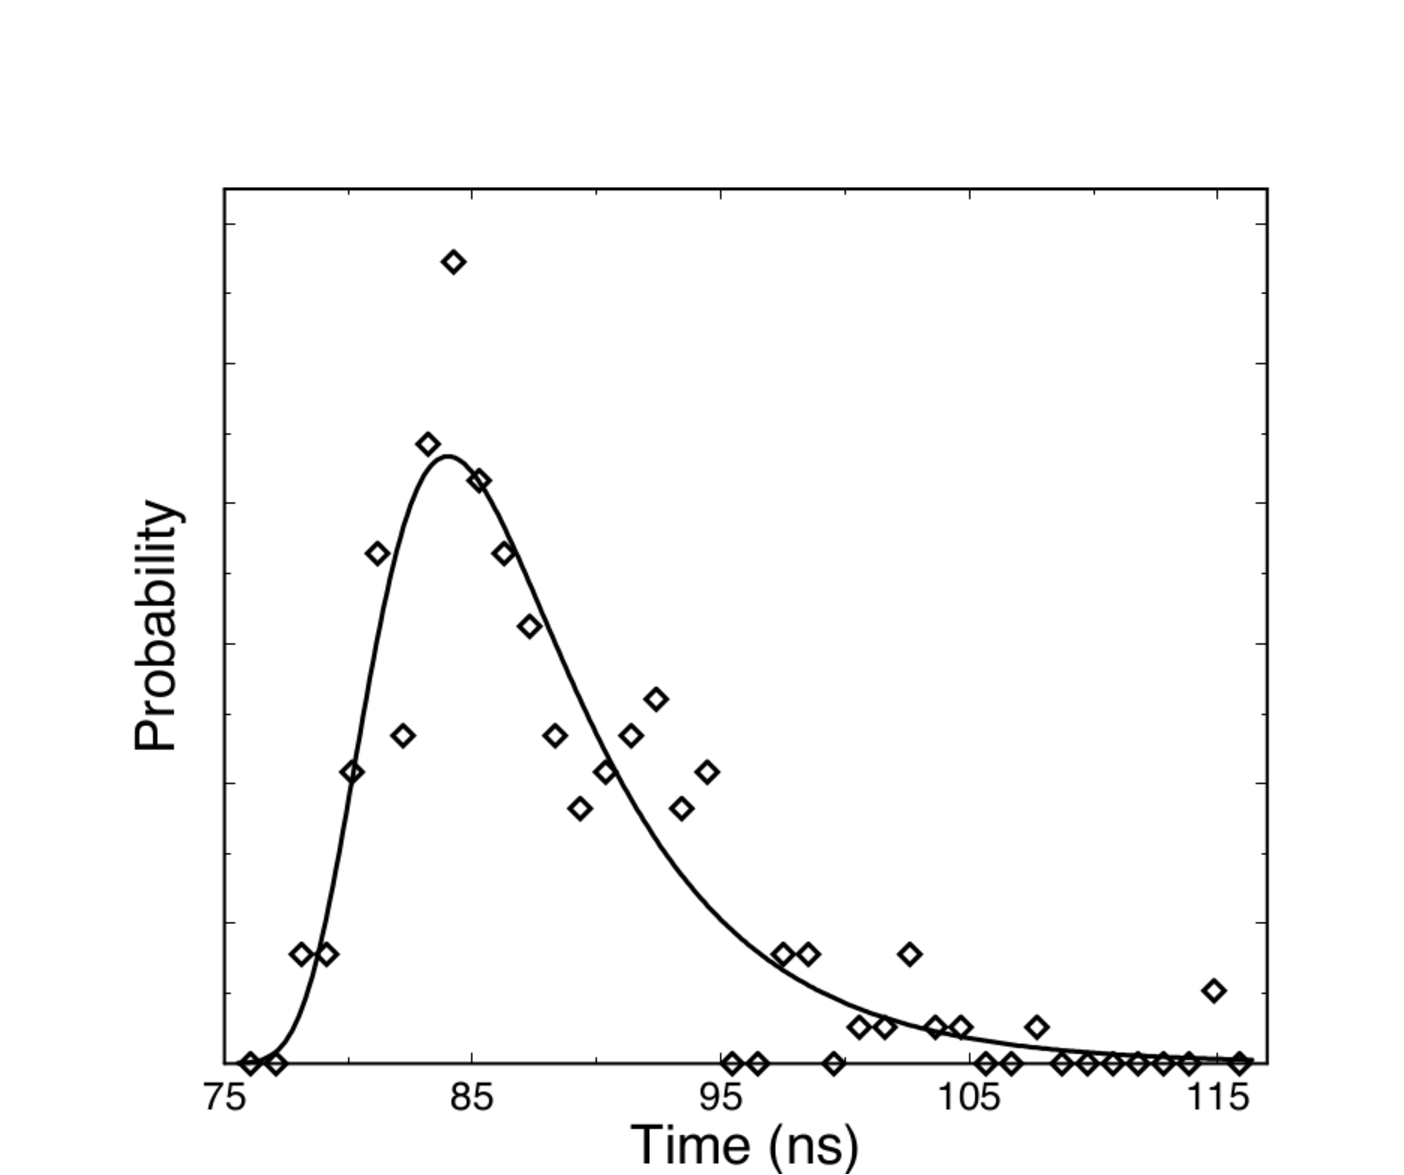
\includegraphics[width=0.45\textwidth]{graficos/fig_9Vis.pdf}}
    \frame{
\includegraphics[width=0.45\textwidth]{graficos/ciclista.png}}
    \caption{Dos figuras contiguas. Las incluimos en un marco para poder mejorar su aspecto.}
    \label{fig:2}
\end{figure}

\end{document}